\let\negmedspace\undefined
\let\negthickspace\undefined
\documentclass[journal]{IEEEtran}
\usepackage[a5paper, margin=10mm, onecolumn]{geometry}
%\usepackage{lmodern} % Ensure lmodern is loaded for pdflatex
\usepackage{tfrupee} % Include tfrupee package

\setlength{\headheight}{1cm} % Set the height of the header box
\setlength{\headsep}{0mm}     % Set the distance between the header box and the top of the text

\usepackage{gvv-book}
\usepackage{gvv}
\usepackage{cite}
\usepackage{amsmath,amssymb,amsfonts,amsthm,mathtools}
\usepackage{algorithmic}
\usepackage{graphicx}
\usepackage{textcomp}
\usepackage{xcolor}
\usepackage{txfonts}
\usepackage{listings}
\usepackage{enumitem}
\usepackage{mathtools}
\usepackage{gensymb}
\usepackage{comment}
\usepackage[breaklinks=true]{hyperref}
\usepackage{tkz-euclide} 
\usepackage{listings}
\def\inputGnumericTable{}                                 
\usepackage[latin1]{inputenc}                                
\usepackage{color}                                            
\usepackage{array}                                            
\usepackage{longtable}                                       
\usepackage{calc}                                             
\usepackage{multirow}                                         
\usepackage{hhline}                                           
\usepackage{ifthen}                                           
\usepackage{lscape}
\begin{document}

\bibliographystyle{IEEEtran}
\vspace{3cm}

\title{1.6.7}
\author{EE24BTECH11002 - Agamjot Singh
}
% \maketitle
% \newpage
% \bigskip
{\let\newpage\relax\maketitle}

\renewcommand{\thefigure}{\theenumi}
\renewcommand{\thetable}{\theenumi}
\setlength{\intextsep}{10pt} % Space between text and floats

\textbf{Question:}
\newline
The value of $m$ which makes the points $\brak{0, 0}$, $\brak{2m, -4}$, and $\brak{3,6}$ collinear, is
\newline
\textbf{Solution:}
\newline
The points $\vec{A}$, $\vec{B}$ and $\vec{C}$ are collinear if
\begin{align}
	\brak{\vec{AB}} &= k\brak{\vec{AC}}\\
	\brak{\vec{B} - \vec{A}} &= k\brak{\vec{C} - \vec{A}}\\
	\brak{\vec{B} - \vec{A}} - k\brak{\vec{C} - \vec{A}} &= 0
\end{align}
Collinearity matrix is given by
\begin{align}
	\myvec{\vec{B} - \vec{A} & \vec{C} - \vec{A}}^\top 
\end{align}
For the vectors $\vec{AB}$ and $\vec{AC}$ to be linearly related, i.e. the points to be collinear, there exists a $k$ which satisfies equation $\brak{4}$.
\newline
Row reduction on collinearity matrix should result in nullity of the matrix to be one, such that some $k$ exists.
\newline
Let the collinearity matrix be $\vec{X}_{m\times n}$.
By rank nullity theorem,
\begin{align}
	\text{rank}\brak{\vec{X}} + \text{nullity}\brak{\vec{X}} = n\\
	\text{rank}\brak{\vec{X}} = n - \text{nullity}\brak{\vec{X}}\\
	\text{rank}\brak{\vec{X}} = n - 1
\end{align}
\newline
Let the points be $\vec{A}\brak{0, 0} \text{,} \vec{B}\brak{3, 6} \text{ and } \vec{C}\brak{2m, -4}$.
The collinearity matrix $\vec{X}_{2\times 2}$ is given by
\begin{align}
	\myvec{\vec{B} - \vec{A} & \vec{C} - \vec{A}}^\top = \myvec{3 & 6 \\ 2m & -4}\\ 
													   &\xrightarrow{R_1 = \frac{R_1}{2}} \myvec{1 & 2\\2m & -4}
													   &\xrightarrow{R_2 = R_2 - \brak{2m}R_1} \myvec{1 & 2\\0 & -4-4m}
\end{align}

For the points to be collinear, the rank of this matrix has to be one.

\begin{align}
	-4-4m &= 0\\
	m &= -1
\end{align}
So, the point $\vec{C}$ is given by
\begin{align}
	\vec{C} = \myvec{-2\\-4}
\end{align}
The line joining $\vec{A}$, $\vec{B}$ and $\vec{C}$ is given by 
\begin{align}
	y &= 2x
\end{align}

\begin{figure}[h!]
   \centering
   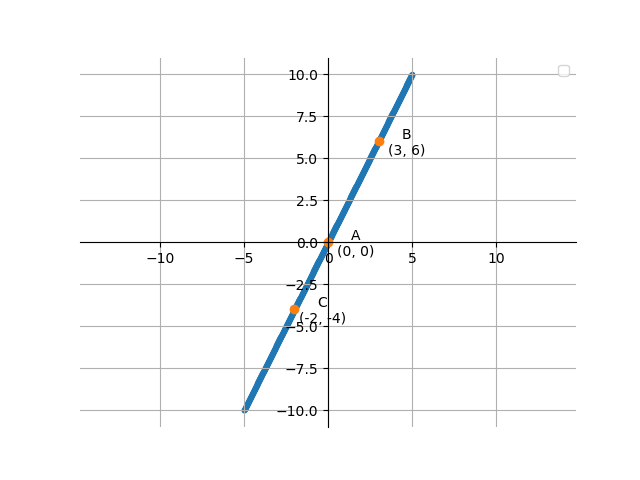
\includegraphics[width=0.7\linewidth]{figs/graph.png}
   \caption{Line containing points $\vec{A}$, $\vec{B}$ and $\vec{C}$}
\end{figure}

\end{document}
